
\chapter{The Science and Nescience of Comparative Linguistics}\label{intro}

\begin{center}
\textbf{Examining the nature and veracity of \textit{Comparative Linguistics} with implications to Aryan-Dravidian hypotheses}
\end{center}

\Authorline{Sudarshan T.N, Madhusudan T.N}


\section*{Abstract}

The two-century-old “field” of study of Comparative (\textit{Historical}) Linguistics (henceforth CL) is critically examined along various dimensions - primarily its evolutionary drivers, the nature of its methods, the supposedly scientific nature of its theories, the assumptions underlying its theories and its socio-political agenda. What are the kinds of questions that Comparative Linguistics tries to ask and provide answers to? Are there alternative approaches and models to engage with these questions? Given the poorly formulated basis of language and its understanding in the West compared to the traditional Indian approaches to language and meaning, are there scientific models of language and language evolution that this field of study is based on? What would the future of Comparative (historical/diachronic) Linguistics look like if this field is given a basis in computational models and frameworks instead of wordlists and theses based on morphology and phonology? What is the traditional Indian perspective on such approaches to theorising about language evolution? As an illustrative case-study (using data) of the larger issues that plague CL, the nature of the Indo-European and Dravidian as language classifications is explicated. Are these language families even valid classifications? We examine many of these issues critically and lay out a comprehensive agenda for a bias-free, scientific and modern Comparative Linguistics.


\section*{Introduction}

\vskip 6pt

Western approaches to understanding the nature of language via linguistics studies and related scholarship over the past few centuries has been without doubt deeply influenced by CL and Philology in its modern avatar - also known as Diachronic Linguistics. The particularly polemic nature of the two century old scholastic pursuit - dozens of Journals, hundreds of books, thousands of linguists, tens of thousands of papers - as attested\endnote{} recently by scholars with backgrounds in the STEM disciplines - is primarily driven by the rhetorical methods of the humanities. From the Introductory article in the new (since 2016) Journal of Language Evolution:

\vskip 6pt

\begin{myquote}
Almost exactly 150 years ago, the \textit{Société de Linguistique de Paris} \textbf{famously banned the study of the origin of language} in the second article of its charter:
\end{myquote}

\vskip 2pt

\begin{myquote}
La Société n’admet aucune communication concernant, soit l’origine du langage, soit la création d’une langue universelle. (The Society does not accept any contribution concerning either the origin of language or the creation of a universal language [translation ours].)(Dediu 2016:1) (emphasis ours)
\end{myquote}

\vskip 3pt

To those engaging with the body of work and scholarship produced by this clique of scholars and also to other interested readers of CL scholarship/papers/arguments - it very much has a veneer of the “scientific” (claims of “proof”, vocabulary – such as trees, genetic relations, clades, comparative method etc). By today’s scientific standards these could at best be classified as superficialpseudo-science methods. Much of the verbal arguments and inferential logic on display in most of these books, handbooks, journals etc. are positioned as deep applications of the “scientific method”. The marked lack of the empirical sensibility, the notions of experiment or of cogent methods of proof is apparent - especially to those from disciplines with more rigour.

We briefly examine the problem of language evolution in general, the origins of this “scholarly” discipline - its motivations and methods. We then illustrate with a few examples fundamental methodological flaws in the techniques used and the dogmas that have evolved as a consequence. The next few sections help develop a narrative - we discuss approaches to the problems addressed by CL, how these problems can be addressed using different paradigms. Approaches which treat Language Evolution as a measurable scientific problem, Computational Modelling, empirical analysis and others are briefly addressed and pointers to a few others are also given. The traditional Indian approach to language and the approaches to linguistics is also discussed.

With this background we then address head-on, the classification of Indo-European and Dravidian as language families. Using insights gleaned from the earlier sections, a balanced critique of CL is presented and pertinent questions raised; the implications to the Dravidian narrative are also discussed. Finally, based on the aforesaid meta-narrative, future directions of research are discussed.


\section*{Foundations}

Language has been deeply studied and explored since earliest times - this much is known. The earliest structured research on language and its origins has been seen in the Vedic / dhārmic traditions. The wide array of analysis and the hoary tradition of language (primarily oral) - the depth of the traditions of \textit{śikṣā} (phonology), \textit{nirukta} (etymology), \textit{chandas} (prosody), \textit{vyākaraņa} (grammar) is astounding and incomparable and as yet not completely fathomed to this day. This body of knowledge, it is to be understood, is not comprised of theoretical structures to be intellectually engaged with, but is scientifically documented, descriptive and prescriptive guidelines to the oral/chanting traditions of the \textit{Veda}. The explicit influence of the “practical” underlies all of the Indic traditions - and language is no exception. The descriptive nature of the language (Sanskrit primarily and also others like Prakrit, Tamil etc) has been captured in efficient (generative) algebraic forms by the earliest scholarship. There is - it is to be noted - no axiomatic basis for language in the Indian tradition. Everything harks back to the \textit{apauruṣeyatva} nature of language deriving from the primordial Veda. There are Greek, Mesopotamian, Babylonian and Chinese linguistics too - but none (to our knowledge) are as sophisticated as the Vedic explanations and related descriptive frameworks. Modern linguistics (particularly in a Western sense) has its origins in the well known Discourse to the Asiatic Society by William Jones (index Jones, William) in 1786. His understanding of Sanskrit and suggestions its commonality with European languages sparked off a feeding frenzy - generations of Western scholars ploughing into Pāņini and the Indian linguistic traditions and “digesting” them into various linguistic theories, methods and frameworks. The famed “philologer” passage is cited below

\vskip 4pt

\begin{myquote}
“The \textit{Sanscrit} language, whatever be its antiquity, is of a wonderful structure; more perfect than the \textit{Greek}, more copious than the \textit{Latin}, and more exquisitely refined than either, yet bearing to both of them a stronger affinity, both in the roots of verbs and the forms of grammar, than could possibly have been produced by accident; so strong indeed, that no philologer could examine them all three, without believing them to have sprung from some common source, which, perhaps, no longer exists; there is a similar reason, though not quite so forcible, for supposing that both the Gothic and the \textit{Celtic}, though blended with a very different idiom, had the same origin with the \textit{Sanscrit}; and the old \textit{Persian} might be added to the same family.” (Burrow Thomas 1973: 6) (index Thomas, Burrow)
\end{myquote}

\vskip 4pt

It is to be noted that there was nothing of note (grammar-wise) in the Western traditions till that time - No systematic grammar, no formal understanding of language despite the so-called Renaissance that had occurred a few centuries earlier. It was the nature of Sanskrit and the advanced understanding of language that sparked off this comparative journey. Despite thousands of years of studying Greek and Latin and centuries of study of European languages, the knowledge of Arabic and other languages, it wasn’t until the European colonizer encountered Pāņini - that the scavenging instincts of the European intellectual collective took over and the feeding frenzy begun.

\vskip 4pt

\textbf{Why was it that the Europeans could not find similar structures in European languages themselves? Why did they need to “compare” it to Sanskrit and other “Indo” languages? Why was there a sudden need to classify European languages now?}

The politics of the era, the predatory nature of Colonialism, the European sensibility conditioned by centuries of Abrahamic polemics are definite reasons. The need to justify the horrors and excesses of colonial behaviour required that the knowledge and traditions of the colonised be shown to be “inferior” or having origins elsewhere - all of this “psychology” is well known and has been addressed elsewhere too. It is being alluded to here simply because it has to be realised that almost all of modern academic discourse and almost all of “scholarship” is still governed by this Eurocentric (western) bias - both in the sciences and in the non-sciences (humanities, social-sciences etc.).

What had passed off as linguistics in Europe was Philology - which has been well analysed and understood as nothing more than tools for socio-political manipulation and rhetoric - flawed manipulative methods masquerading as a science. Philology’s origins in organised religion and socio-political motivations are well understood. For a history of Philology in the West see (Turner 2015), for balanced critiques from a traditional (\textit{sanātana}) viewpoint see (Narendran, T.M. 2017) (Sudarshan T.N. 2017). Modern linguistics discourse has nearly succeeded in “digesting” much of the Sanskrit tradition; so much so that there is almost no sign of “Sanskrit” in the modern linguistics discourse. The World Atlas of Language Structures does not even have an entry for Sanskrit.

\begin{myquote}
The World Atlas of Language Structures (WALS) is a large database of structural (phonological, grammatical, lexical) properties of languages gathered from descriptive materials (such as reference grammars) by a team of 55 authors. (2017, wals.info)
\end{myquote}

Even taking a non traditional stance - ignoring the notion of \textit{apauruṣeyatva} - the origins of language are still unknown and are mostly speculative in nature. The origins of speech both from a cognitive and physiological dimension are unknown. The origins of writing systems are pretty much unknown too. Coulmas (2008) in his book addresses the evolution of writing systems in detail. It is to be noted that there are \textit{Vedic} hymns which mention writing both directly and indirectly - so the notion of writing as a later development is largely speculative. The \textit{Yajur Veda} (\textit{Taittirīya samhitā}) has references to numbers, fractions. Such intricacies are not possible without the corresponding written symbols. There are references to writing and symbols in the Atharva Veda too. The origins of the domains of discourse on language - that of meaning and semantics - are also pretty much speculative. How does meaning evolve? What are the forces that underlie the creation of structures in language which correspond to meaning? None of these is known and almost all of our (western) knowledge on these core fundamentals is speculative at best. Given the extremely shaky foundations of almost all of the key issues underlying language - it is interesting to know that modern (Western) linguistics and most notably CL has successfully orchestrated theories of human migration, human behaviour and continues to influence supposedly scientific fields like Population Genetics, Cognitive Science and more. Biological, physiological, social, socio-psychological dimensions to these questions also need to be addressed. None of these can be answered without proper modelling and simulation studies. The nature of methods used by CL scholarship - fragile (low dimensional) methods using morphology and phonology - word list comparisons, speculations on phonetic evolutionary paths which comprise the Comparative method has been critiqued by many index Niyogi, Partha) (Niyogi P. 1995, 1998, 2002, 2009) (Subrahmanya, K. 2008) (Dediu, D. \& Boer, B.D. 2016) from different standpoints - each of them coming at CL theories from varying backgrounds; we shall briefly discuss these critiques in later sections.


\section*{Motivations of Comparative Linguistics}

The origins of CL are well understood and documented. There is lots of historical material detailing its evolution in the past two centuries (Brugger 2003) (Clackson 2009)(index Clackson, James) (Hope \& Joseph 2014) (Lehmann \& Winfred 2010) and much more. Lehmann’s work (in our opinion) is sufficiently detailed (historical perspectives) and has a relatively low polemic factor.

The well known origins are alluded to; it is to be noted that parallel interests were also present among German scholars.

\begin{myquote}
The Asiatic Society of Bengal, at whose meetings its founder, Sir William Jones (1746–94), 1 delivered his influential lectures, was established in the aim of pursuing those investigations. At the same time the Romantic Movement, especially in Germany, \textbf{devoted considerable attention to the study of earlier periods, at least in part on the grounds that knowledge of simpler eras would assist an understanding of the culture of their own time.} (Lehmann 2010:13) (emphasis ours) (index Lehmann, Winfred)
\end{myquote}

The possibility of a “family” of languages was intriguing - simply because the new language (with associated works of grammar and descriptive theories) was from a “non-European” area and by non-European peoples \textbf{(Why was there no scholarship/interest in studying commonalities in languages (comparative linguistics), before discovering Panini?)}; the predatory nature of colonial European scholarship was kindled - and techniques and methods to “digest” the body of knowledge were developed over the next centuries.

\begin{myquote}
Such motives led to one of the most fruitful intellectual pursuits of the nineteenth century - the \textbf{investigation of the numerous languages of the Indo-European language family and determination of their background, ultimately also of the language of a preliterate period now referred to as Proto-Indo-European. } (Lehmann 2010:13) (emphasis ours)
\end{myquote}

The Colonial nature of the times and the racist motivations of Colonisation (exploitative commerce, mindless loot, proselytization) as expected did affect the motivations of study. Colonisation was being justified in the guise of “civilising” efforts - the well known “white-man’s burden”- so it was essential that “cultures” of the others be studied; (as we know now) primarily to help in the efforts of whitewashing history. Edward Said’s (index Said, Edward) body of work is very well illustrative of this. The initial aims (as in many scholarly pursuits) were lofty; after the initial efforts, much of the “deep” and fundamental aims were cast aside - and the aims became far narrower.

\begin{myquote}
The \textbf{principal aim of Indo-Europeanists throughout the nineteenth century then came to be far narrower than that of the founders of the field.} It was directed largely at the languages. Descriptions of the individual languages, and comparative studies with statements on interrelationships among them, as well as on their groupings, were not only the chief aims of Indo-European studies, but also the primary contributions of the century. (Lehmann 2010:14) (emphasis ours)
\end{myquote}

\newpage

Much of the initial work was abandoned - new definitions were proposed. (It is noted that this is after a few decades of study of Pāņini in Europe - the general scholarship began to understand the approach and the genius of the Indian grammarians). It is interesting to note that the “historical” dimension was actually abandoned,

\vskip 2pt

\begin{myquote}
That attitude led to \textbf{restatement of the phonology, the grammar, and the lexicon, with ever greater restriction of aims; extensive monographs were now published that dealt with specific sets of forms, such as the perfect (Osthoff 1884). Profiting by this achievement, the generation after Bopp's death set out to treat the original language much like languages spoken today, applying methods that they considered as reliable as those of the physical sciences.} (Lehmann 2010: 18) (emphasis ours)
\end{myquote}

\vskip 2pt

The pseudo-scientific approach - and the search for universal laws had begun. The issues in applying “current” laws to historical conditions were glossed over by later scholarship and the scholarly community in general.

\vskip 2pt

\begin{myquote}
\textbf{… they sought to deal with language much as their colleagues in the natural sciences dealt with their selected topics.} In their day the faculty of philosophy had not only developed much more widely than had the other three traditional faculties — law, medicine, theology — but it also came to be fragmented. Its major components were labeled "the natural sciences, " which \textbf{treat those areas where universally valid laws apply}, and "the historical sciences, " where generalizations apply differently in different periods and differing societies; (Lehmann 2010: 19) (emphasis ours)
\end{myquote}

\vskip 2pt

Whatever were the changes in the first few decades - the deeper “orientalism” did not change much.

\vskip 2pt

\begin{myquote}
Besides directing attention to spoken language, Brugmann set as one of the goals of linguistic study the \textbf{"attainment of a deeper understanding of the mental activity of human beings in general and of the individual Indo-European peoples"} (Lehmann 2010:22) (emphasis ours)
\end{myquote}

\vskip 2pt

\begin{myquote}
That is to say, for Brugmann at this time \textbf{actual contemporary speech, not abstract or classical patterns, is to be investigated to achieve an understanding of language.} And since language has a twofold aspect — mental as well as physical — such study increases our understanding of its speakers. Moreover, in his view \textbf{linguistic study contributes to an understanding of society and groups within it.} (Lehmann 2010:22) (emphasis ours)
\end{myquote}

The Neo-Grammarians (so called because of their axiomatic (assumptions based) approach to grammar) slowly started having influence in the humanities too - little of the scientific approach was seen.

\begin{myquote}
While the two important principles of the neo-grammarians are irreproachable, and while he recommended attention to contemporary languages, there is \textbf{no denying that Brugmann and his colleagues devoted themselves almost entirely to the study of languages of the past. Even works like Paul's German grammar treat the language in its historical development.} But it should also be clear from Brugmann's statement of principles that the \textbf{aims of the neo-grammarians as he stated them are almost ideal for pursuing study in the humanities.} (Lehmann 2010:23) (emphasis ours)
\end{myquote}

Early twentieth century saw some important \textit{cultural} interpretations based on CL methods which even in those biased times was found to be inappropriate. The language based theories of culture, migration and prehistoric theories were loose and speculative.

\begin{myquote}
.. the work of \textbf{the late nineteenth-century prehistorians came to be more and more rejected.} The large work dealing with many facets of culture, including such practices as music, that was assembled to celebrate the seventieth birthday of Hermann Hirt (1936) may be occasionally mentioned still, but is today not accorded much credence. (Lehmann 2010:35) (emphasis ours) (index Lehmann, Winfred)
\end{myquote}

\begin{myquote}
In short, \textbf{the aim to determine the culture of the Proto-Indo-European community was vigorously pursued for some time, but the conclusions were held to resemble fiction more than fact.} As a further result, they did not contribute to solving the problem of the homeland. \textbf{Greater assurance came to be expected from the rapidly developing field of archaeology.} (Lehmann 2010:35) (emphasis ours)
\end{myquote}

Though the culture and origins of PIE people, anthropological claims of PIE etc. were dismissed by scholars (at the turn of the twentieth century) - lot of it has resurfaced in the mid and late twentieth century and is pretty heavily in use by scholars and pseudo-scholars who make a living of Indian socio-political churnings. The last few decades has seen lots of pseudo-scholars both of Indian origin and others have been resurrecting these theories of Aryan homeland, Aryan origins, Aryan Invasion/Migration theories, Dravidian origins of India and much of the deeply flawed discourse in popular mainstream media channels. Both of the so-called left and right voices indulge in these laborious theorising and exercises in pontification based on these pseudo-theories. Breathless quoting and re-quoting by linguists/scholars have kept much of these speculations alive.

A sober analysis of the field will highlight that much of the methods and conclusions are driven by selective data, arbitrary methods and flawed interpretations. We shall discuss some aspects of this in the next sections.

\begin{myquote}
While the \textbf{handbooks of Brugmann, Delbrück and Meillet among others can scarcely be surpassed as sources for data and their interpretation at the time each of these works was published, the new data coupled with expanded methodological procedures require revised interpretations and updated handbooks for the dialects at the early period and for the proto-language itself.} The aims of Indo-European linguistics today then parallel those of the beginnings of its study, \textbf{but extend over many more facets of the language and the culture thanks to vastly increased information and the impressive results of virtually two centuries of study.} (Lehmann 2010:44) (emphasis ours)
\end{myquote}


\section*{Methods of Comparative Linguistics}

We now examine the approaches used and methods of doing CL. We track the historical evolution and motives and how they have influenced the methods over the years. The Proto-language reconstruction was one of the principal preoccupations. Sanskrit could not be the “influencer” of European languages. It had to be something else. This was the primary axiom. We quote from Gamkrelidze and Ivanov’s well appreciated and recognised tome on Indo European linguistics.

\begin{myquote}
Among the favorite themes and \textbf{main tasks of linguistics from the last century to the early years of this one were questions of the reconstruction of Proto-Indo-European}, and in the world's universities the chief, and usually the only, linguistics department was a department of comparative Indo-European linguistics. It was \textbf{that epoch whose efforts are summed up in the classic handbooks, efforts directed at revealing the diverse particulars of the common proto language} underlying the genetically related members of what is known as the Indo-European linguistic family.(Gamkrelidze et.al 1995:xix) (Foreword by Roman Jakobson) (emphasis ours)
\end{myquote}

This book is considered to be a wide ranging interdisciplinary work. In the field, its erudition is considered to be unsurpassed. Many of the views are also deemed to be controversial (their proposal to place the \textbf{\textit{Urheimat}} of the IE people south of Caucasus for example) within the field.

\begin{myquote}
The approaches to particular problems of \textbf{Proto-Indo-European linguistic antiquity taken by researchers from around the world are brought to bear here, and an appealing answer is given to the various theses that entered scientific currency at the turn of the century. This work stands out not only for its unusual answers to old questions, but in the very way it poses questions and the unprecedented breadth of its thematic horizon.} (Gamkrelidze et.al1995:xx) (Foreword by Roman Jakobson) (emphasis ours)
\end{myquote}

The preoccupation of the theories to identify culture of the speakers of the fictitious PIE - the PIE people underlies all of Indo-European CL.

\begin{myquote}
Consistent with the \textbf{dialectic removal of the dichotomy of synchrony and diachrony and with the parallel inclusion of spatial diffusion among internal linguistic factors, the book naturally transforms the time-honoured, spatially and temporally uniform view of Proto-Indo-European and creates a model of dynamic synchrony which fully comprehends the foundations of the proto- language, its evolutionary shifts, its internal, regional differentiation, and its recurrent intersections with neighbouring linguistic areas.} It is the questions of mutual interactions among the dialects of Proto-Indo-European and the relations of the protolanguage to neighbouring protolanguages \textbf{that have given rise to the authors' richly promising work on the geographical definition of the (Southwest Asian) Indo-European homeland and the early migratory routes followed by the various branches of Proto-Indo-European.} (Gamkrelidze et.al1995:xix) (Foreword by Roman Jakobson) (emphasis ours)
\end{myquote}

The principal method or “algorithm” in the arsenal of the CL scholar is the Comparative method and Reconstruction. This is also noted in Saussure’s classic “Course of General Linguistics”

\begin{myquote}
The sole means of reconstructing is by comparing, and the only aim of comparison is a reconstruction. \textbf{Our procedure is sterile unless we view the relations of several forms from the perspective of time and succeed in re-establishing a single form.}
\end{myquote}

\begin{myquote}
\textit{Ferdinand de Saussure, Cours de linguistique generale}\\\textit{(transl. Wade Baskin)}(Gamkrelidze et.al1995:5) (emphasis ours)
\end{myquote}

Once language “features” are compared and if absent reconstructed (entire languages are reconstructed), the method that follows is that of typology, the classification of languages according to structural and functional features.

\begin{myquote}
\textbf{Typological verification} raises the probability of reconstructed phonemic and morphological patterns, and permits changing the reconstruction from a mere numerical catalogue into a \textbf{more realistic portrayal of the linguistic system.}
\end{myquote}

\begin{myquote}
\textit{Roman Jakobson, Typological studies and their contribution to historical comparative} linguistics (Gamkrelidze et.al 1995:5) (emphasis ours)
\end{myquote}

The book captures the inner workings of the mind of the CL scholar. What are called facts are actually “assumptions”. Recreating structures of fictitious languages that connect to existing languages (by some typological reasoning) are driven by pre-existing motives.

\begin{myquote}
… the book presents the results of linguistic analysis - phonological, morphological, syntactic, and areal-dialectological - of Proto-Indo-European. This does not mean that the analysis should be viewed as a systematic survey of the various branches of comparative Indo-European grammar, as is done in the standard handbooks. Rather, the first part is a \textbf{study of key questions of Proto-Indo-European structure, involving a wide range of facts and yielding a relatively complete picture of this language in its dynamic development and its typological links to other language systems.} (Gamkrelidze et.al1995:vii) (emphasis ours)
\end{myquote}

Much of the field was influenced by developments in Science at that time. Much of the vocabulary and methodology were influenced by the efforts in the Physical sciences, primarily ideas from biological classification. The evolution of the methods in CL is described by Lehmann (Lehmann 2010:8),a theoretical evolution with very little evidence from actual language “instances”. Without data, proof or empirical evidence, primarily based on verbal rhetoric the methods of CL propound theories of PIE. We had earlier indicated that the Reconstruction and typology methods are amenable to back fitting any structural change in any direction to fit any evolutionary theory.

\textbf{Example:} Did short \textbf{e} become long \textbf{e} or was it the other way round or did both happen/exist in parallel? Was there a normal ‘e’? Was there a high pitch \textbf{e} or low pitch \textbf{e}? What about combinations in pitch and stress? The reconstruction methods of CL assume whatever fits into the larger theory that the scholar wants to create - this is how all of the theories and evolution trees are “generated”. Ideally there should be some amount of probabilistic modeling of the evolutionary paths and there would be some amount of math behind these assumptions.

Sadly - the entire field of CL is math-free and model-free.

Say Xa, Xb, Xc are three samples of linguistic data - where X is a language feature, and a, b, c are 3 different existing languages

\textbf{Comparative Method} is brought to play where existing data from different languages (at least 3) are compared, their differences are duly noted:Xa, Xb and Xc are now known to be different in some ways (say phonologically or morphologically or whatever)

The second-step is \textbf{Internal reconstruction}. Depending on which direction one has pre-decided the “evolution” one assumes the evolution in that direction If one wants to “show” Xa and Xb came from Xc or from some fictitious Xx then internal reconstruction is used to show evolution in that direction. The “steps’ in the reconstruction may not be real, as seen in the \textbf{“e”} example.

\textbf{Typological reconstruction} is used across these languages (both real and fictitious) to “create” families: Classes of features and feature values are “combined” in convenient ways to form language families.

Entire fictitious languages can be created and the cultures of their speakers also “reconstructed”!

\begin{myquote}
\textbf{In sum, historical linguists have at their disposal three methods: CM, IR and glottochronology. Of these CM is most highly regarded and most widely used; but it can be applied only when data in three or more related languages are available. IR has been applied with impressive results, but the data needed for its use in a language are often unavailable. Glottochronology has severe limitations. Besides these methods, historical linguists make use of the findings of typological study, both to identify patterns that provide possibilities for explanation and patterns that lend credence to conclusions that have been advanced through application of the three methods.} Linguists have always examined their conclusions with reference to patterns in other languages; but the patterns so used have often been atypical, taken from languages that the individual happened to know. The findings of typological study are based on examination of all languages for which data have been secured; accordingly, they provide much more secure bases for such purposes. (Lehmann 2010:74) (emphasis ours)
\end{myquote}

The flaky nature of the principal methods that underlie CL have been hinted at.We recommend serious readers to “walk-through” some of these handbooks to understand the “free-for-all” that passes for “method”.

\textbf{\textit{Phonology-}} based classification in CL has been influenced by the “root” theory from Panini’s descriptive grammar via Sausserean grammar discourse. The notion of Paninian ‘Guna’ digested and recast as “Grade’ becomes a critical dimension on which Phonology based classification happens (ablaut, umlaut are notable examples). Use of Internal reconstruction, typology fitting and choices of arbitrary evolution direction are blatantly apparent. The ablaut phenomenon is a classic example of all these “dubious” methods in action in Phonology. See (Lehmann 2010:147,151,178,179).

Similar “modus” is seen in the use of \textbf{\textit{Morphology}} features.The partially digested “\textit{kāraka}” is seen in action in various half baked forms is used to classify morphological features.Verb derivation, verb suffixes, verb affixes, tense, categories of person etc. are also considered to be morphological features of interest. See (Lehmann 2010:215,242).

Once the basic features of Phonology and Morphology are \textit{taken care} of by CM and IR - what remains is \textbf{\textit{language syntax}}. This set of features (both in a diachronic and synchronic sense) is in reality a “dynamic” feature. With regard to spoken language, the various accents and dialects of a language are primarily variances of syntax. Features of Syntax are critical when it comes to analysis of “written” language. We show in a later section that much of the assumptions of sentence order (possibly the most important syntax feature) is also a “weak” feature from an evolutionary perspective and cannot be used as a dependable marker. Analysis of the Lexicon - the dictionary of words in a language forms the largest set of “data” - introduces the semantic dimension to CL. Again Lehmann acknowledges the influence of Sanskrit -though we do not see this in the standard handbooks. Nouns, Noun forms, Kinship terms (Szemerényi’s research), Social organisation, Numerals, Compounds and the use of Onomastic Indexes are also used as targets for application of the methods. Lexicons especially are liberally interpreted in the PIE speculations.

\begin{myquote}
\textbf{.. noted that examination of the words used in daily affairs permits identification of subclassifications in the lexicon. Forms of such everyday words are often inflected in accordance with procedures that have been superseded, as in Proto-Indo-European by the thematic inflection. Examination of the lexicon then assists us in singling out words that may reveal an earlier form of the language and through reconstruction of it insights into the culture and society of the speakers at an earlier time. Analysis of the lexicon in this way provides one of the three bases for determining that culture, and for further inferences, such as the likely homeland of the speakers.} Combined with data provided by archaeological discoveries, and by scrutiny of early texts, the lexicon has been examined for more than a century for evidence it contains to determine the culture of the Indo-European peoples and their early location. (Lehmann 2010:380) (emphasis ours)
\end{myquote}


\section*{The Nescience of Comparative Linguistics}

We examine the premises and principles that underlie diachronic linguistics. The key exercise of “\textit{reconstruction}” that scholars perform along various dimensions is largely, the fantastical science in CL. The “Scholarship” is discussed under 5 principal types of reconstruction (Gamkrelidze et.al 1995).The typological verification of reconstruction, reconstruction of sound, reconstruction of semantics, entire reconstructed systems and finally the reconstruction of original language and original territories.

\textbf{Typological verification} is used as a tool to classify families. The fundamental aspects of feature design and directionality of evolution are not considered to be “verifiable” artefacts. It is only the “classification” and groupings of features that is to be verified. The only check in the reconstruction process is actual language data. In their absence a free-for-all results and the resulting inference is arbitrary. In the case of the Dravidian Family tree there are actually multiple layers of reconstructed language families. The so-called check by universals is sufficiently “lax”. The universals themselves are based on European languages and the already pre-assumed nature of language and its structures. Much hubris can be seen in the discussion on diachronic transformations (i.e arbitrary evolution of a language feature in time and space), they are compared to be as powerful as generative grammar just because they derive from some theoretical construct. As we indicated above - the theoretical “basis” is already created based on European perspective of language. See (Gamkrelidze \& Ivanov 1995:75,76,77) for examples of the overall circular dependencies of Typological verification of language reconstructions. Methods for phonological (\textbf{sound}) reconstruction have a few assumptions. Again there is nothing to indicate that this is the ideal formulation of the problem space - we had suggested probabilistic models previously. Again, we can see pseudo-scientific reasoning underlies the sound reconstruction paradigms. (Gamkrelidze et.al1995:79). Similar observations apply for \textbf{semantic} reconstructions too, mostly composing of verbiage; no models, no math underlie any of the formulations. See (Gamkrelidze et.al 1995:83). While discussing entire \textbf{reconstructed systems}, the overall flakiness and the pseudo-scientific become very obviously apparent.

\begin{myquote}
\textbf{A reconstructed linguistic model reflects a protolinguistic system which once existed, and the time frame within which it existed and changed must be reconstructed, as must the geographical aspects of its spread. If a protolanguage is regarded as a system which existed in space and time and had a history, then the dynamics of its evolution must be studied and account must be taken of its earliest scientifically recoverable stages and its history up to its breakup into could be syllabic or not depending on context, will be defined as [+ syllabic, + nonsyllabic]: daughter dialects and their formation as independent linguistic units. Many structural properties of Proto-Indo-European which are reconstructed in classical Indo-European studies as static schemas can be broken down into chronological stages.} Features which are reconstructed for an undifferentiated source system often do not belong to the late period of its development and dialectal differentiation but reflect an earlier stage. This explains the frequent debates in Indo-European comparative grammar over linguistic structures that appear mutually exclusive; an example is the discussion of the number of laryngeals in Indo-European, where each of the several incompatible solutions has good evidence in its favor. \textbf{In such instances the various solutions can be associated with different developmental stages of PIE, which permits us to regard many of the proposed structures as chronologically complementary and datable to different stages.} (Gamkrelidze et al 1995:84) (emphasis ours)
\end{myquote}

\begin{myquote}
\textbf{The motionless, static PIE scheme must be replaced with a chronologically dynamic system, one which, like any attested language, had its history and evolutionary dynamics. That history presupposes both internal evolution of the system and areal associations with other systems, reflected in contacts and interference.} In this respect we can speak of linguistic borrowings into PIE from other languages and from PIE into other languages which were in contact with it.. (Gamkrelidze et al 1995:84) (emphasis ours)
\end{myquote}

The primary motives of CL, the need to locate \textbf{origins of people} from whom Europeans possibly descended have its own set of assumptions driving the PIE homeland theories. Assumptions of single origin for language, similar to single origin hypothesis for human evolution underlie much of PIE theorising and forms the \textit{apex} of the nescience of CL.

\begin{myquote}
A group of related languages is formed when an original linguistic system disintegrates due to disruption of contacts between speakers of individual dialects; the languages are spread to their historically attested territories by migrations of the speakers. \textbf{This means that the original range of the common source linguistic system lay in a particular area, an area more compact than the range of the daughter languages, from which the out-migrations originated.} (Gamkrelidze et al 1995:86) (emphasis ours)
\end{myquote}


\subsection*{Discussion}

The preceding section highlighted the peculiarly idiosyncratic nature of the methods of CL. (Niyogi 1995:200) explicitly identifies this problem in his work on models of language evolution. The assumptions implicit in the derivations based on language features drive the evolution trajectory and the resulting language family classification.

In the previous sections we have detailed the methods underlying the linguistic scholarship over the past two centuries. Using Gamkrelidze and Ivanov’s seminal book as basis - we have examined some core issue in methodology and approach. The lack of an empirical basis or even a basic model which captures some sort of evolutionary dynamics is lacking. The complete reliance on verbal argumentation and the lack of any sort of formalism - is from a scientist's perspective - a serious flaw in the approaches pursued in this area of study. Almost all areas of non-trivial scholarship have evolved to have basis in at-least some (mathematical or otherwise) models. For a large scale, complex, nonlinear dynamic phenomena like language evolution - reliance on 18th century polemicised verbal-style reasoning is something truly astonishing. A more detailed (empirical) analysis of the “descriptive” approaches used by linguists is provided in a separate section where we discuss the data provided by the World Atlas of Language Structures.

It is indeed surprising that this has not been called out by honest incisive scholarship. Given the multidisciplinary nature of the problems being addressed and the momentum of two centuries of scholarship, it is definitely not easy. A recent journal that specifically addresses these issues - Journal of Language Evolution (first issue in January 2016) - does indeed recognise this. In the journal’s opening article -

\begin{myquote}
We believe that probably the most important development in the field of language evolution of the last decades has been \textbf{the full recognition that we need to base our theorizing on \textit{actual data} (or to formulate it more negatively, that speculation unfounded in data is no longer acceptable) and the realization that we can in fact \textit{collect} such data in a controlled and principled manner. Moreover, there has been great progress in tools to \textit{analyze} the complex kind of data that we need to deal with.} (Dediu2016:2) (emphasis ours)
\end{myquote}

Unless, there is verifiable proof for theories posited which are based on non-trivial models (statistical or otherwise) it is difficult to accept verbal arguments - that have been the basis of linguistics scholarship for centuries.

\begin{myquote}
We believe that a \textbf{proper understanding of such present-day data is the only valid path toward a science of language evolution,} and it is this belief that justifies the contents of the first issue of this journal featuring an introduction to linguistic diversity, a debate on the effects of climate on current linguistic diversity, and an introduction to cutting-edge statistical analysis of experimental results from living humans. (Dediu 2016:2) (emphasis ours)
\end{myquote}

The attempt in this section has been to examine the core assumptions that directionalize the field of Comparative Linguistics. The principles and assumptions that govern the methodologies that drive the scholarship - those that have resulted in two centuries worth of theorising have been highlighted. Attempts have been made to identify not only the glaring internal inconsistencies of these assumptions but also the nescience of the overall “humanities-driven” rhetorical approaches. The current approaches in CL provide minimal checks on the endlessly dizzying assumptions that scholars have been making; one theory after the other - all based on “imagination”. Yes, hypothesising and imaginative leaps of faith are part of the scientific process but they need to be backed by experiments and models which have the ability to explain and predict - none of these “scientific” features are present in CL - they are not even discussed.


\section*{Alternate approaches to Language and its Evolution}

\subsection*{Swadeshi Perspectives}

As seen in the preceding section, many principal assumptions and methodologies that underlie Indo European classification; their methods and motivations drive primarily from Panini’s work -the concepts of \textit{guņa} (forms/grades), \textit{vŗddhi}, \textit{dhātu-s} (stems/ roots), \textit{kārakas} and much more. None of these constructs nor anything close to techniques similar to the methodology of Panini was even present in “western scholarship” until that time. Carried away by the imperialist motives and the prevalent feeding frenzy (of Panini) - basic ideas were mangled, modified and new theories constructed around them - all the while the motivations being to show that the European “peoples” and languages had nothing to do with either the language of Sanskrit or the peoples who spoke them - hence the “pursuit” of homeland theories and theories of migration (which actually have nothing to do with language evolution in a scientific sense). Two unrelated fields of study were juxtaposed - to serve the (Abrahamic) European civilizational need of \textbf{conquest} and \textbf{othering} - driven by the motives of the deeply racist societies of the times. The crown-jewel of these theorisations - the proto language formulations - is probably the epitome of these vacuous theories. It is critical for the Proto-IE-language theorising that the so-called \textit{Vedic Sanskrit} be dated as 1500 BCE; the clade/ family of languages that Indo-European is supposed to comprise will not allow for earlier dates. Figuratively speaking - \textbf{\textit{the entire house-of-cards will come crashing down.}}

We now present a novel formulation, to help understand the CL \textbf{“\textit{kurukṣetra.}”} The entire CL enterprise over the past two centuries and more has been theory building - with the following three principal classes of motives:

\newpage

\begin{enumerate}[{\rm 1)}]
\itemsep=0pt
\item Theories to make Sanskrit as distant (in the tree model of languages) as possible from European languages

 \item Theories to “speculate” and “manufacture” a common (common to Sanskrit and European languages) ancestor language

 \item Theories to speculate and manufacture the origins of the peoples of this “ancestor” language to be in Europe (preferably Western Europe). 

\end{enumerate}

\textbf{Class 1} can be seen if one were to examine the methodologies and vocabulary of CL. Almost all of the techniques are “digested” from work of Panini and the Sanskrit grammarians - they have been given different names and methods mangled and the Sanskrit origins removed from the discourse. Other than some of the handbooks - almost all of the literature on languages ignore “Sanskrit” as being the source of linguistic ideas. See (Subrahmanya 2008) and (Jha 2010) for the Sanskrit tradition. See (Saussure 2013) for a “excellent sample” of digestion in action. All the formal paradigms of Modern linguistics (which are heavily influenced by Sanskrit), chose to ignore the work of the various Indian grammarians and any discussion even of Panini, Patanjali or Bhartrhari.

\textbf{Class 2} can be seen in scholarship pertaining to the comparative method and the proto-language theories; the entire 2nd volume of Gamkrelidze and Ivanov’s seminal book comprises this - details of proto Indo-European language, the culture of the speakers and their lifestyle etc. An unknown/unspoken language and fictitious people are explained in excruciating detail. This piece of scholarship very much represents and demonstrates the deep seated collective ego of the “Western Universalist” narratives that is mainstream today. This narrative has hardly been challenged. Even the voices in the West (new journals, computer scientists, geneticists etc.) which oppose these theories do so only tangentially - they do not address the origins of these theories or their history and their hegemonic nature. The result is carry-over vocabulary and implicit assumptions - case in point; it is very much apparent in much of population genetics research, names of language families and speculations with basis in CL carried over to form basis of the structural and geographic vocabulary over which findings and new theories (based on gene data) are posited. That the underlying assumptions are themselves erroneous and representative of western hegemony - is something that will not be acknowledged unless addressed directly (a task for Swadeshi Indology).The need to continue with the hegemonic truths is civilizational, deep-seated and will require serious challenge from alternative worldviews (Swadeshi perspectives for example). This peculiar sort of theorising and whitewashing of history is also seen in the West-centric historiography of the sciences and mathematics - so - the historiography of linguistics and languages is not a unique case. Groundbreaking scholarship by Rajiv Malhotra (Being Different 2013) and others have highlighted this in detailed terms and provoked fundamental shifts in perspective.

\textbf{Class 3} Scholarship is the entire range of theories speculating on the population origins and peopling of India. (Invasion and migrations theories of various sorts are an ever popular genre of scholarship). That such a culture (Indian) (superior in every known dimension) could be present in the world (Sanskrit being representative of this “superiority) at a time when European collective ego had to be supreme - was not possible. Spectacular theories were offered as part of nineteenth century scholarship - both in the humanities and sciences and continue mostly unchallenged, to this day. The effects are seen today; scholarship in many areas like population genetics wherein the famed Sforza paper (Cavalli-Sforza, 1988, 1997) has been influenced by this discourse and it in turn continues to influence Class 3 scholarship.


\subsection*{Western Linguistics}

Western (linguistics) scholarship does indeed acknowledge the limitations of these descriptive approaches. \textbf{\textit{Kees Versteegh}} one of the editors, is quoted in his contributory piece “\textit{The study of non-Western traditions}” in Volume 3, \textit{History of Language Sciences} and makes the case for going back to the traditions. Why do we study Linguistics in India (origins and evolution our own languages) using methods invented with European languages at the core? The strange pursuit of “Comparative Linguistics”, is also acknowledged not to be part of any tradition, including that of the classical European, but grew out of the societal needs of 19th century Europe. The nature of the global discourse has deeply affected linguistics scholarship worldwide. So much so, that the term \textit{linguistics} is even considered to apply only for the peculiar 19th century European enterprise. The roots of CL in this enterprise have been discussed in previous sections. There is nothing universal or globally applicable in much of the scholarship that underlies CL. The Linguistics traditions throughout the world - had their own approaches - local to their needs and specific to their cultures - and the generalisation of theories happened with their tradition at the core. Comparing languages was a peculiar European exercise - acknowledged here. This is the case in Indian Linguistics too. The “linguistic” traditions in Sanskrit and the other languages of the subcontinent traditionally had their own forms and methodologies. (Auroux 2000:2792)

The Indo-European family classification and Dravidian families are “products” of this Western hegemony - they are not the traditional perspective, nor are they based on universal principles, nor are they scientific. Caldwell’s “Dravidian” work is very much of the “missionary grammar” genre as alluded to below.

\begin{myquote}
As a result of \textbf{the hegemony of Western European culture, Greco-Latin grammar eventually became the canonical model for the description of the world’s languages. Thus, most of these languages were described by an exogenous model that had originally been elaborated for a different language.} Most attempts to describe a language with the help of a foreign model aimed at creating a contrastive grammar for learning purposes. The use of an exogenous model in itself does not preclude an accurate analysis of the linguistic data. \textbf{This is particularly clear in the case of the missionary grammars that described the ‘exotic’ languages with which Europeans came in contact.} (Auroux 2000:2794) (emphasis ours)
\end{myquote}

The primary reasons for the thrall of Western models of linguistics in Indian Universities and in mainstream discourse is the lack of promotion or recognition of the traditional perspectives (not to mention general \textit{tamas} and incompetence). The colonised University Education system of independent India has not helped either. Almost all (dozens of them) Linguistics departments in the country operate using these western models - When will they wake up?

The Indian tradition of linguistics is rich and varied and has its own models, motivations and goals. These perspectives ought to aid the linguistic studies in India. If Indians don’t do Indian linguistics the Indian way, who will? The search for universals and interpretation of the World’s languages ought to happen based on the basis of a core Indian tradition. When is this going to happen? Does Indian scholarship even realise the deep issues that remain to be identified - leave alone addressed. Actual Linguistics aside - even the history of linguistic study and languages does not have a “swadeshi” \textit{dṛṣṭi} in Indian academia and scholarship - and is under free interpretation by Western Linguists and Indologists. So - How do we address these fundamental issues? To begin with - by at least recognizing that we are doing linguistics using (colonized) imported models. Sadly, other than Professor Korada’s phenomenal work (Subrahmanya 2008) (index Subrahmanya, Korada) there is very little of note from Indian scholarship either to counter the thrall of the West or correct the \textit{dṛṣṭi} by engaging with western models rooted in Indian linguistic traditions. The Indian linguistic tradition is rooted in Dharma (good language leads to \textit{Dharma)}.The aim of language is to help dhārmic living.

We see this fundamentally “\textit{swadeshi}” notion expressed by the Sanskrit Grammarians.

\begin{myquote}
Katyayayana and Patanjali vociferously express this view at the outset of mahabhasya - \textit{siddhe śabdarthasambandhe lokato rthaprayukte śabdprayoge śastreṇa dharmaniyamah} - \textbf{\textit{Vyakarana} can be written when sabda, artha and their relation follow a standard, and the task of Sastra is to notify/prescribe that a certain form of a sabda, which is already used in a particular artha by people, if employed, would render dharma ( implying that the opposite would give adharma).} (Subrahmanya 2008:3) (emphasis ours)
\end{myquote}

Grammar (Sanskrit grammar particularly) has dual purpose in the tradition - elucidation of meaning and dharma.

\begin{myquote}
One can compile a \dev{व्याकरणम्,} if and only if the \dev{शब्द, अर्थ} and their \dev{सम्बन्ध} are immutable / eternal. Unlike in other languages \dev{संस्कृतम्} has got two purposes - \dev{अर्थप्रत्यायनम्} and \dev{धर्म।} (Private Email with Prof. Korada Subrahmanya)
\end{myquote}

The Grammar of the Tamil language has hoary history too. There have been many Tamil grammars. See (S. Subramanya Sastry 1997) for fascinating history of the Tamil Grammatical tradition.Scholars are asked to juxtapose this with the CL driven Dravidian history of Tamil language from (Subrahmanya Sastri P.S. 2008). The contrast is stark. Mainstream discussion of Tamil and the language is always coloured by the CL theories and speculations - but nothing could be further from the truth. The “power” of the CL narratives has been on display during much of the years of the Dravidian movement. The interpretive power provided by Caldwell’s theses and the seemingly powerful explanatory power of CL methodology has deeply buried - both from academic scholarship and Tamil discourse - the traditionally known history of the Tamil language.

Almost all of the Tamil grammarians (there are around 15 major Tamil grammarians listed by Subrahmanya Sastri) have their unique imprints in documenting the historical evolution of Tamil language through grammar. They date from pre-Common Era right up to the 18th century CE. None of them use any of the methods of CL or of any of the theories of CL. The influence of the Sanskrit Grammarians can be seen - not only in the style of compilation but also in the use of grammatical theories. The earliest known - the Tolkāppiyam - definitely shows influence of the models of the \textit{Prātiśākhya-s}, Yaska’s \textit{Nirukta}, Panini’s \textit{Śikṣā} and \textit{Vyākaraņa} and even some of those of Panini’s predecessors.

All of this only suggests the shallow nature of the methodology and claims of CL and as a result - the classification of Dravidian and Indo-European. The false divide between Indian languages was purely a colonial exercise in divide-and-rule and something which has been continuing even 70 years after Independence. Modern Indian linguistics scholarship has not addressed these issues head-on. What could be the reasons? There seems to be no motivation to have any sort of “swadeshi” \textit{dṛṣṭi}. The thrall of the coloniser and his models of analysis and interpretation still looms large - especially so in the humanities and linguistics departments.

Much of these “\textit{swadeshi”} perspectives, goals and aims are totally alien to Western linguistic thought as yet. The notion of \textit{dharma} at the core of language theory is intrinsic to the “swadeshi”/\textit{sanātana} nature / \textit{dṛṣṭi} and is something that cannot be replaced by western notions of language. There are other dimensions to language namely the psychological, the energy (vibrational) dimensions seen and experienced in the transformative powers of chants, \textit{śloka-s, mantra-s} which form the principal basis of the Veda - Āgama tradition.

These are areas of analysis and study which cannot even be attempted if we were to base linguistic study on Western universals. Neuro-biological analysis (instrumented measurement and statistical studies) is one way to empirically assess the experiential claims of the tradition. There are no models - either of a mathematical or theoretical (verbal) nature to explain or even describe these phenomena (vocabulary, ontology, descriptive models etc.) to make them amenable available for scientific validation approaches. Design and development of hypotheses and novel experiments based on a deep understanding of the traditional models of mind is one possible way forward, before one could attempt any sort of theorising.


\subsection*{Scientific Approaches to Language Evolution}

Previous sections hinted at the weakness of the science behind much of CL - its methods, approaches and inferences. The key problem that CL aims to solve is the dynamic nature of language evolution. What would a scientific approach look like? Partha Niyogi’s research suggests many alternatives. (Unfortunately he could not continue his research as he passed away in 2010.) Language evolution is a dynamic non-linear phenomenon. Techniques from Learning theory, statistical and computational modelling are brought to bear upon this problem of language evolution. Specific evolution “phenomena” are modelled and the validity of the modelling approach is illustrated. The rationale for a computational modelling approach is provided by Niyogi. (Niyogi 2002:1) and (Dediu 2016:3) (index Dediu, Dan) discuss this in fairly comprehensive terms.

So, what are these models? There are many already in use now and many new ones need to be developed.

\begin{myquote}
There are \textbf{many examples of excellent computational models to select from}, and we can illustrate the width of approaches with just a few: there is of course Lieberman and Crelin’s (1971) classic computational study of Neanderthal \textit{vocal abilities}, which has engendered a literature of its own, the latest instalment probably being Badin et al. (2014). A different computational tradition uses agent-based models to study how language emerges in societies of artificial agents, including the influential \textit{iterated learning} (e.g., Smith, Kirby, and Brighton 2003) and Steels’ (1995), \textit{language game} models. \textbf{There are also models of a more mathematical nature, such as those inspired by theoretical biology proposed by Nowak and his students (e.g., Nowak 2006). Yet another class is exemplified by Dunn et al.’s (2011) use of Bayesian phylogenetic models inspired from evolutionary biology to investigate language change.} (Dediu 2016:3) (emphasis ours)
\end{myquote}

Language evolution - as we have tried to show, is a complicated problem space. The number of factors governing it and the dimensionality being addressed is large. Simplistic low dimensional assumptions and manual verbal reasoning (comparative method, internal reconstruction etc) trivialise the problem. These arcane methods should be abandoned for any true scientific pursuit of CL.

\begin{myquote}
Inquiries into language origins and evolution have always drawn upon several disciplines at once, but the last few decades have seen an explosion in the breadth and depth of such collaborations between disciplines. The discovery of \textit{FOXP2} and the continued exploration of its functions, evolution, and relevance for language and speech can serve as an example. \textbf{It involves molecular genetics, evolutionary genetics, bird song biology, language and speech pathology, cognitive neuroscience, linguistics, archaeology, paleoanthropology, and paleoecology, not to mention sophisticated computer models required for analysis.} (Dediu 2016:3) (emphasis ours)
\end{myquote}

This field is truly multi-disciplinary and requires the brightest from all fields to engage in constructively without resorting to the tiring old polemics. There are deeper issues in this space; Journals and the momentum of two centuries of scholarship and current practitioners of these “old” methods, cannot be wished away. They exist and need to be engaged with “scientifically”. Prone as they are as a community to vociferous polemics and averse to anything that resembles “math” or “science”- this real-world aspect cannot be ignored. The future of Language Evolution research is indeed interesting. See (Dediu2016) for a detailed analysis.


\section*{The IE and Dravidian Classification}

The previous sections discussed CL and its methods and a preliminary critique was presented. More analytical critiques will be offered in the Appendix on WALS data. A “swadeshi” perspective to the problems and recommendations for a “swadeshi” \textit{dṛṣṭi} was offered. It is with this background that one should approach the Dravidian language family classification too. The existence of Journals of Dravidian Linguistics, the state funded Dravidian University, the state funded Central Institute of Classical Tamil and the numerous departments of Dravidian languages and linguistics in Indian universities exemplify this - the intellectual colonization is extremely deep.

We recommend study of Appendix - 1 of (Subrahmanyam, 2008:295..334) for a reader on the evolution of the Dravidian formulation. Whyte Ellis’s (index Ellis, Whyte)speculation of a “South Indian” family in the Introduction to a 1816 book on Telugu Grammar by Alexander Duncan Campbell and(index Campbell, Alexander) its christening as “Dravidian” by Robert Caldwell in 1856 mark the beginnings. The “migration” theories, Aryan migration/invasion and anti-Brahmin rhetoric is ever-present - but all of that is well known. Much of Caldwell’s book uses methods made popular by the German comparative-linguists of that era. There is also speculation using data from Greek geographers and merchants (place names, mountains etc.). Caldwell (index Caldwell, Robert) speculates on everything - Tolkappiyam, Thirukkural, Tamil inscriptions, Telugu, Malayalam, Canarese (Kannada) - he had something to say on most south Indian linguistic artefacts known during his time. Given his background as a man of the Church - his motives to find division in society was through the varņa and jāti identifiers. North India was already sufficiently divided using religion as a wedge - So how were North and South Indians to be divided? How were South Indians to be divided amongst themselves? Enter the “Dravidian”.

The Aryan and Dravidian language family was convenient in many ways, to the political needs of the Empire, the needs of the men of the Gospel, to European ethnographers and historians who needed a \textbf{\textit{cultural source for Europe older than the Assyrian}} and to the various European Nationalisms.

\begin{myquote}
\textbf{The hypothesis of the existence of a remote original affinity between the Dravidian languages and the Sanscrit, or rather between those languages and the Indo-European family of tongues, inclusive of the Sanscrit, of such a nature as to allow us to give the Dravidian languages a place in the Indo-European group, is altogether different from the notion of the direct derivation of those languages from the Sanscrit.} The hypothesis of a remote original affinity is favoured by some interesting analogies both in the grammar and in the vocabulary, which will be noticed in their place. (Caldwell 1856:29)(emphasis ours)
\end{myquote}

The seeds for contemporary Dravidian identity politics and the continuing socio-political upheaval since the last century in the Tamil land were sown by Caldwell’s speculations.

\begin{myquote}
\textbf{In Tamil, on the contrary, few Brahmans have written anything worthy of preservation. The language has been cultivated and developed with immense zeal and success by native Tamilian Sudras; and the highest rank in Tamil literature which has been reached by a Brahman is that of a commentator.} (Caldwell 1856:34) (emphasis ours)
\end{myquote}

Much of Caldwell’s book is organised around methods used by linguists in Indo European works, Phonology, Morphology, Inflexion analysis, pronoun analysis, Case analysis etc. As much linguistics work continued after Caldwell, in order to fit in inconsistencies and various data the standard methods of creating new intermediate languages was adopted. The Dravidian Family of languages has its own elaborate Proto-language tree - Proto-Dravidian, Proto-South Dravidian, Proto South-Central Dravidian, Proto-Tamil-Kannada, Proto-Telugu, Proto-Tamil-Toda, Proto-Kannada, Proto-Tamil-Kodagu, Proto-Tamil-Malayalam, Proto-Tamil. This proto-tree is the result of decades of application of the CL methods. See (Krishnamurti 2006: 21) for a family tree of the Dravidian languages. Dravidian linguistics scholarship has speculation that goes the other direction too - the influence of the Dravidian on Indo-Aryan.

\begin{myquote}
Thus the Dravidian grammatical impact on Indo-Aryan has been far greater than the Indo-Aryan grammatical impact on Dravidian – a point that specialists on Indian linguistic history seem not to have appreciated. How can we account for this pattern? \textbf{Even after three millennia or more of Indo-Aryan-Dravidian contact the Dravidian languages have changed relatively little in their grammatical structure, whereas Indo-Aryan has undergone major grammatical restructure.} (Sjoberg 1992:524) (emphasis ours)
\end{myquote}

All the critiques that apply to the Indo-European linguistics also apply to the Dravidian linguistics. The methods used are the same - the comparative method, internal reconstruction and speculative evolutionary paths. The methods are deeply flawed and the conclusions are hardly scientific, there are no models nor are there any predictions. All the issues that we have seen apply to CL in general also apply to Dravidian in particular. In short - the IE classification is flawed and so is the Dravidian.

All the critiques on the methodologies and foundations apart - Are these two so called different families really that different? We present (in the Appendix) an analysis of data of these two families in the to highlight flaws, using the “expert” data provided by the linguists themselves.


\section*{Discussion and Perspectives - Looking ahead}

In the preceding sections we have made the case for analysing Comparative Linguistics from its sources; What were the origins?, What was its evolution, its goals, motivations?, What were the methods used?. A deep understanding of these led to a appreciation of the problem space of CL - what is now also known as “Language Evolution”. The models and assumptions of CL are peculiar to 19th Century Europe. Modern scholarship (including those of western linguistics) appreciates the limitations of the approaches. The vocabulary and linguistic family classifications still influence current research in linguistics and also in other fields like population and evolutionary genetics. The momentum of centuries of research and the hegemonic nature of the discourse is not easy to counter. Language and Linguistics has to be rid of these classifications, vocabulary and has to adopt scientific approaches which are tighter and verifiable. Scholarship from other fields have to understand and appreciate the genesis, the nature of CL and refrain from using these CL “inferences” and vocabularies as frameworks to base their favorite migration or evolution theses. Much of this has been seen in recent decades in evolution and population research based on genetic data.

The evangelical and colonial basis of the “Dravidian” classification and its continuing usage in polity both in Tamil Nadu and in the larger “\textit{Breaking India”} machinations is understood but does not have popular awareness - mostly, because of the manipulative “education” content and the sheer will and momentum of those in power. The Schools, Colleges and Universities across Tamil Nadu primarily subscribe to the theories and ideologies of those in power and play a major role in the perpetration and sustaining of these divisive identities. They are very much part of the problem themselves and should preferably not be looked at for solutions.

The Dravidian classification and the related linguistic theories are based on the methods developed in Indo European linguistics. Much of these methods are flawed and can be considered minimally scientific (if at all).The theories and inferences arrived at using these methods are questionable and should be ignored in any future scholarship.

The traditional Indian approach to linguistics is (as is known) much different. Neither “Language evolution” nor the existence of different languages was considered a “problem”. No theories were needed to explain it. These were considered to be local cultural artefacts that mostly evolved \textbf{in-situ}. India’s spectacular linguistic heritage attests to this. The Sanskrit and Tamil grammar traditions have each co-evolved and should continue to do so using modern tools and techniques. It is indeed distressing that not much of note has happened either in Tamil or in Sanskrit grammar-wise in the past two centuries to counter the CL discourse. The synthetic approach of Indian knowledge systems does not allow for the reductionist/comparative approaches to language just for the sake of it - there has to be a dhārmic (\textit{prayojana}) reason.

Empirically speaking (at high resolutions) every person’s grammar (spoken and written) is different. It is only on this basis only that we are able to identify “signatures” based on voice and text data. These are techniques used in advanced security and surveillance systems. Just because grammars are different or unique does not mean it is to be “separated” and “classified” and made into families - not to mention the search for who influenced whom and where they all come from.

As is seen, even in preliminary computational models using data from the recent few centuries (data from English and French) - even the principal “markers” of a language (according to CL) such as sentence order (SOV or SVO,.. ), features of phonology and morphology change drastically within a few generations of speakers and \textbf{the “directionality” of change is purely arbitrary.} These are “deep” CL notions essential for the theorising of evolution and the “generation” of complicated family trees. The inferences from these computational models strike at the root of the assumptions of CL. The evolutionary directions are nothing more than wishful thinking. Pick any arbitrary direction of change (phonological) for a vowel or consonant or even morphological - we have different evolutionary trees. See (Niyogi 1995) (index Niyogi, Partha) for the example using \textit{French} and (Niyogi 2002) for the example using \textit{English}. The directionality is sufficiently arbitrary and has serious implications to the entire pursuit of Proto-language design. Even based on an initial analysis - we feel that almost all of the proto language theorisations are simply arbitrary.

A more detailed critique of the arguments and disassembly of the handbooks (the mainstays of the theories) in CL need to be done - and obviously more research and scholars are needed. This preliminary (but fundamental) analysis should - we hope spark interest in more “\textit{pūrva pakṣa}”. More scholars with multidisciplinary skills (computer science, programming, linguistics, math at the least) are essential. Much of CL handbook data (laboriously crafted over the past two centuries) once made available in “machine readable” formats will make research much easier and amenable to the application of data-science methods. These can be used to analyse the “rigor” of the CL theories and also can help in the design of the computational models of language evolution. Existing problems can be framed within these models and hypotheses tested based on actual data - instead of depending on “\textit{hand-waving} vigour” methods of “scholarship”. As an illustrative example of this approach, preliminary analysis of data from WALS is provided in the Appendix.


\section*{Concluding Remarks}

This paper is a preliminary attempt by us to highlight the deep issues arising out of accepting in good faith - theories of the Colonisers - in this particular case - those of Comparative Linguistics. True de-colonisation will happen only when we question and deconstruct the assault on identity. Sadly, intellectual colonisation is still deep rooted. The linguistic classification of Indo-European and Dravidian has been mostly unquestioned. Little of note has been forthcoming from traditional scholarship in this area of comparative linguistics. The relentless colonisation of University resources and the onslaught of western universalism, not to mention the impact of the “Dravidian” movement have caused much of Indian and in this particular case Tamil society to accept blindly - categories and classification thrust on them by invaders and foreigners. This is pretty much to script (as also seen in the in different continents that have been assaulted by Colonisation) - the frontal attack of Colonisation is the attack on identity.

The very essence of being Indian is actually being questioned in much of Tamil society. The Dravidian movement and its leaders have effectively used these theories for usurping power and for self-aggrandisement. The Dravidian movement having its origins in the Justice Party (anti-India, anti-North, anti-Gandhi, anti-Brahmin ideologies) being at its core, carries much of the divisive seeds of dissent, sown during the colonial period. This has also enabled the evangelical and proselytising forces to operate with impunity and with success in much of Tamil Nadu.

It is pretty much acknowledged that the seeds of these “separatist” tendencies lie in the notion of a linguistic identity (Dravidian) that is decidedly separate from the rest of India. This has led to socio-cultural fissures in Tamil society. The need to examine the roots of this “linguistic” dimension, led us to study the nature of \textit{Comparative Linguistics}. We have, we believe shown that almost all of the theories and methods underlying CL are questionable and mostly unscientific. The theory that is the result of these methods - the classification of Dravidian as also the formulation of Indo-European language families has been examined and is found to be severely flawed. To allow such theories to flourish and influence (the millennia old) Tamil society is truly deplorable. We hope that this initial effort encourages future empirical scholarship in language evolution.


\section*{Appendix - WALS Data Analysis (index World Atlas of Language Structures)}

\subsection*{Background\protect\endnote{}}

\begin{itemize}
\item The currently known Global Data Sources for language

\end{itemize}

There are currently two global-scale continually maintained inventories of the (signed and spoken) languages of the world:

\textbf{Ethnologue (18ed):} \url{http://www.ethnologue.com} contains speaker numbers, detailed locations, and other metadata

\textbf{Glottolog (2.6):} \url{http://www.glottolog.org} contains sources of data on languages and a more principled

\begin{itemize}
\item The currently known Global Data Sources for language evolution

\end{itemize}

The following is a selection of databases of worldwide scope which are publically available and accessible and cover the domains of phonology, lexicon, and grammar respectively:

\newpage

\textbf{PHOIBLE \url{ http://phoible.org}:}

PHOIBLE Online is a repository of cross-linguistic phonological inventory data, which have been extracted from descriptive sources. The 2014 edition includes 2, 155 inventories covering 1, 672 distinct languages.

\textbf{ASJP \url{ http://asjp.clld.org/}:}

The Automated Similarity Judgment Program (ASJP) has a database of 40-item word lists of basic vocabulary for 6895 varieties covering 4, 401 distinct languages. The word lists are transcribed in a simplified but uniform transcription system.

\textbf{WALS \url{http://wals.info}:}

The World Atlas of Language Structures (WALS) has 192 multistate grammatical features sparsely filled in for 2, 679 languages. A subset of 200 languages is densely filled in. The features were individually designed by experts on the respective domain of grammar (and binned into maximally six feature values owing to the original publication as an atlas with no more than six colors on a map).


\subsection*{Analysis}

Data from the WALS source is analysed and some results presented. We present only a few preliminary observations here.

\begin{enumerate}[{\rm 1)}]
\itemsep=0pt
\item \textbf{Total number of languages:} 2679 (language Nandi, row number-1666 does not have wals code)

 \item \textbf{Total number of families:} 256 families (unique family names)

 \item \textbf{Total number of unique values for genus:} 544

\end{enumerate}


\subsection*{1. Feature Analysis}

\begin{itemize}
\item \textbf{Total number of features:} 192 (202 columns, out of which, 10 are not features)

 \item \textbf{Feature type:} Categorical

 \item \textbf{Possible values that the features can take are given at this \url{https://docs.google.com/document/d/1HCdjZoyIjX9k9JH5mJUSXXnEiVeTDzagyyzo6aMPySA/edit?usp=sharing}:}

 \item \textbf{Distance measure:}

\begin{itemize}
\item 
 \textbf{Issues Faced}

 Distance between two vectors X and Y is given by sum(|Xi-Yi|) where i denotes the feature ‘i’th. How do we deal with a NaN? Assuming that a NaN \textbf{(Not a Number)} occurs when the that particular question is not relevant to the language, two languages having a NaN for a field can be taken as zero, what about the case where one is NaN and the other is not?

\begin{figure}\end{figure}

 \item 
 \textbf{Approach taken}

 Assign integral values to NaN categories 1, 2, 3 etc. when doing detailed analysis.All attributes can be taken to be equally important in the initial iteration of the analysis.

\end{itemize}

\item \textbf{List of number of languages per family can be found here:} \url{https://drive.google.com/file/d/0By1QhePejHuGYjZxMEhQOXd2eEk/view?usp=sharing}

 \item \textbf{List of number of non-NaN features per language:} \url{https://drive.google.com/file/d/0By1QhePejHuGMjZsQk85dkVhZFU/view?usp=sharing}

\end{itemize}

\textbf{WALS classifies the features into the following (\url{http://wals.info/feature}):}

See area column on the link in the subheading, click the drop down to get various options

\begin{itemize}
\item Phonological - 20 features, Sign languages - 2 features, Others - 2 features, Morphology - 12 features, Nominal categories - 29 features, Nominal syntax - 8 features, Verbal categories - 17 features, Word order - 56 features, Simple clauses - 26 features, Complex sentences - 7 features, Lexicon - 113 features

\end{itemize}


\subsection{Illustrating Data Sparsity (weak basis for models for Comparative Studies)}

Dark value in the matrix plot below indicate a feature with a non null value. If the entire feature set were present for each language one would have a completely black rectangular matrix.

\begin{figure}[!hbp]
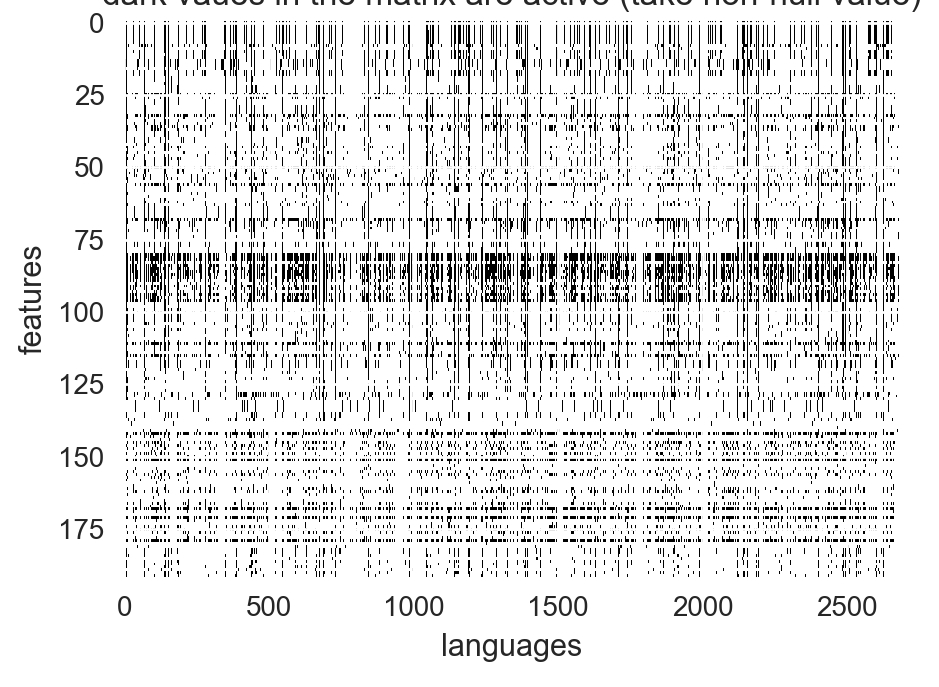
\includegraphics[scale=0.29]{"images/6_02.jpg"}
\caption{Figure 1: Plot of Language features and language}\label{art6-fig02}
\end{figure}

The number of cells in the matrix = features x number of languages = 192 x 2679 = 514368. Number of empty cells = 437903. \textbf{85.13 \%} of the cells are empty.

\textbf{What does this sparsity indicate?}

It can indicate two things.

\begin{enumerate}[{\rm 1)}]
\itemsep=0pt
\item Feature data not available for language X

 \item Feature not present for language X

\end{enumerate}

If it is the former, then we need to wait for updation of the database. More likely it is the latter. The sparsity (approx 15\% filled) indicates something about the quality of feature design. Ideally a feature should be something that is common across all sample classes. One should be able to compare “similar” instances and show difference in “values” of that feature. Not the presence or absence of that feature.

\textbf{Example:} If one were to compare and classify “fruits” a feature would be \textbf{COLOR} - so Apple has {color=red}, Orange has {color=orange} would be feature values. One would generally not design features like “\textit{Redness}” or “\textit{color same as name}”. Such feature designs (features which are unique only to one or very few classes) generally lead to sparseness of feature data.

Language classification is done on the basis of these features. The sparse nature of the “comprehensive” WALS data glaringly indicates the overall lack-of robustness / feasibility of the features designed used in language classification.

\section{2. Examining Indo-European and Dravidian Families}

\begin{figure}
\caption{Figure 2: PCA plot of first two features of WALS. Dravidian (blue), IE (Red) and Niger-Congo(black)}
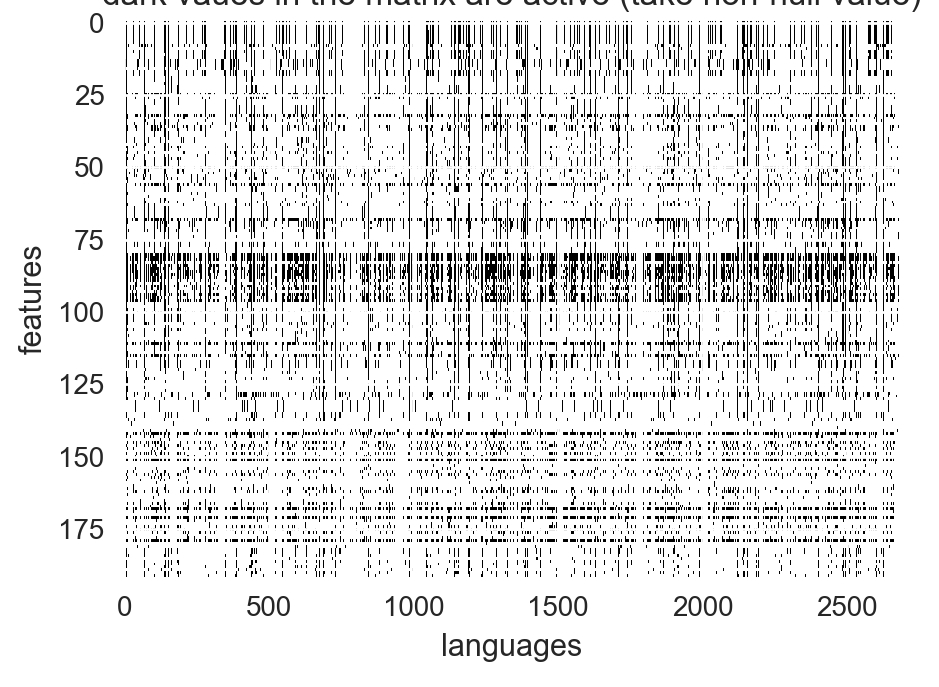
\includegraphics{"images/6-02.jpg"}
\end{figure}

\textbf{Observation:}

In the PCA (\textit{Principal Component Analysis i.e. the principal components, the most influential features which enable classification}) plot, the first two features account for only 60\% of the variance in data. Generally, it is much higher. We are not sure of the inferences we can derive from PCA on this data.

There are some languages across the three families, which are close. But overall, there seems to be distinction between Niger-Congo vs Indo-European and Dravidian families, but the difference is not clear between the Indo-European and Dravidian families. Comparing IE and Dravidian languages, one feature at a time, only some of the word order based features showed statistical similarity. (Only those features that had a probability of having non-null value in at-least 35\% of languages in both the families were considered). More Plots (across all features) are being worked on and shall be made publicly available.


\section*{Acknowledgements}

The authors wish to thank Prof. Korada Subrahmanyam, affiliated to the University ofHyderabad, for many incisive discussions on the traditional Indian approach to Linguistics.


\section*{Bibliography}

\begin{thebibliography}{99}
\bibitem{006-key01} Andronov, Mikhail Sergeevich (1977) \textit{Dravidian Languages}. Vijayawada. Visalandhara Publishing House

 \bibitem{006-key02} Auroux, Sylvain (2000) \textit{History of the Language Sciences = Geschichte Der Sprachwissenschaft = Histoire Des Sciences Du Language: An International Handbook on the Evolution of the Study of Language from the Beginnings to the Present...} Berlin: De Gruyter.

 \bibitem{006-key03} Bowern, Claire \& Bethwyn Evans (2015) \textit{The Routledge Handbook of Historical Linguistics}. New York, NY: Routledge.

 \bibitem{006-key04} Brügger, Michael Meier, Matthias, Fritz and Manfred Mayrhofer.(2003) \textit{Indo-European Linguistics}. New York, NY: Walter De Gruyter.

 \bibitem{006-key05} Burrow, Thomas (1973) \textit{The Sanskrit Language}. London: Faber and Faber.

 \bibitem{006-key06} Caldwell, Robert A. (1868) \textit{Comparative Grammar of the Dravidian or South-Indian family of Languages}. London: Trubner \& Co

 \bibitem{006-key07} Cavalli-Sforza, Luca Luigi and Feldman, Marcus W. (1981) \textit{Cultural Transmission and Evolution: A Quantitative Approach}. Princeton: Princeton UP.

 \bibitem{006-key08} Cavalli-Sforza, L. L., Piazza,A., Menozzi, P. and J. Mountain. (1988) "Reconstruction of Human Evolution: Bringing Together Genetic, Archaeological, and Linguistic Data." \textit{Proceedings of the National Academy of Sciences} 85.16: 6002-006.

 \bibitem{006-key09} Cavalli-Sforza, Luca L. (1997) “Genes, peoples, and languages”. PNAS 1997. 94: 7719-7724

 \bibitem{006-key10} Cavalli-Sforza, Luca, L. and Mark Seielstad (2001) \textit{Genes, Peoples and Languages}. London: Penguin.

 \bibitem{006-key11} Clackson, James (2009) \textit{Indo-European Linguistics: An Introduction}. Cambridge: Cambridge UP.

 \bibitem{006-key12} Coulmas, Florian (2008) \textit{Writing Systems: An Introduction to Their Linguistic Analysis}. Cambridge: Cambridge University.

 \bibitem{006-key13} Dawson, Hope and Joseph, Brian D. (2014) \textit{Historical Linguistics}. New York: Routledge.

 \bibitem{006-key14} Dediu, Dan and Bart de Boer. (2016) “Language evolution needs its own journal,” \textit{Journal of Language Evolution}, Volume 1, Issue 1, 1 January 2016, Pages 1–6, \url{https://doi.org/10.1093/jole/lzv001}

 \bibitem{006-key15} Fábregas, Antonio, Jaume Mateu I Giral, and Michael T. Putnam.(2015) \textit{Contemporary Linguistic Parameters}. London: Bloomsbury Academic.

 \bibitem{006-key16} Fox, Anthony (2007) \textit{Linguistic Reconstruction: An Introduction to Theory and Method}. Oxford Textbooks in Linguistics: Oxford UP.

 \bibitem{006-key17} Gamkrelidze, Tamaz Valerianovič., Vjačeslav Vsevolodovič Ivanov, and Werner Winter.(1995) \textit{Indo-European and the Indo-Europeans: A Reconstruction and Historical Analysis of a Proto-language and a Proto-culture}. Berlin: Mouton De Gruyter.

 \bibitem{006-key18} Greenberg, Joseph Harold and William Croft. (2005) \textit{Genetic Linguistics: Essays on Theory and Method}. Oxford: Oxford University.

 \bibitem{006-key19} Greenhill, S. J., Q. D. Atkinson, A. Meade, and R. D. Gray.(2010) "The Shape and Tempo of Language Evolution." \textit{Proceedings of the Royal Society B: Biological Sciences} 277.1693: 2443-450.

 \bibitem{006-key20} Harris, Roy, Talbot J. Taylor, Nigel Love, and C. H. M. Versteegh. (1997) \textit{Landmarks in Linguistic Thought}. London: Routledge.

 \bibitem{006-key21} Holdcroft, David. (1991) \textit{Saussure Signs, System and Arbitrariness}. Cambridge: Cambridge.

 \bibitem{006-key22} Jha, V. N. (2010) \textit{Language, Grammar and Linguistics in Indian Tradition}. New Delhi: Munshiram Manoharlal Pvt Ltd

 \bibitem{006-key23} Jones, Charles (2014)\textit{ Historical Linguistics Problems and Perspectives}. London: Routledge.

 \bibitem{006-key24} Koerner, Ernst F. K. (1971) \textit{Ferdinand De Saussure: Origin and Development of His Linguistic Theory in Western Studies of Language. A Critical Evaluation of the Evolution of Saussurean Principles and Their Relevance to Contemporary Linguistic Theory}. Braunschweig: Vieweg+Teubner Verlag

 \bibitem{006-key25} Krishnamurti, Bhadriraju (2006) \textit{The Dravidian Languages}. Cambridge: Cambridge.

 \bibitem{006-key26} Lehmann, Winfred P. (2010) \textit{Theoretical Bases of Indo-European Linguistics}. Florence: Taylor and Francis.

 \bibitem{006-key27} Malhotra, Rajiv (2013) \textit{Being Different: An Indian Challenge to Western Universalism}. Noida: Harpercollins India.

 \bibitem{006-key28} Mallory, J.P. and Adams, D.Q.(2009) \textit{The Oxford Introduction to Proto-Indo-European and the Proto-Indo-European World}. Oxford: Oxford.

 \bibitem{006-key29} Millar, Robert McColl, and Trask, Robert L. (2015) \textit{Trask's Historical Linguistics}. London: Routledge.

 \bibitem{006-key30} Narendran, T.M. (forthcoming) \textit{A Parīkṣā of Sheldon Pollock’s Three Dimensional Philology}. Chennai: Infinity Foundation India.

 \bibitem{006-key31} Niyogi, Partha (2002) "The Computational Study of Diachronic Linguistics." \textit{Syntactic Effects of Morphological Change}: DOI:10.1093/acprof:oso/9780199250691.003.0020

 \bibitem{006-key32} Niyogi, Partha, and Berwick, Robert C. (1997)"A Dynamical Systems Model for Language Change." Complex Systems, Vol 11, Issue 3, 161-204

 \bibitem{006-key33} Niyogi, Partha (1998) “The Logical Problem of Language Change”. In: \textit{The Informational Complexity of Learning}. Boston: Springer.

 \bibitem{006-key34} Niyogi, Partha (2005)."Theories of Cultural Evolution and Their Application to Language Change." In Briscoe, Ted (Ed.) \textit{Linguistic Evolution Through Language Acquisition.} Cambridge: Cambridge ebooks. Pp. 205-34.

 \bibitem{006-key35} Niyogi, Partha (2006) \textit{The Computational Nature of Language Learning and Evolution}. Cambridge, MA: MIT.

 \bibitem{006-key36} Nowak, Martin A., Komarova, Natalia L. and Partha Niyogi (June 2002). “Computational and evolutionary aspects of language.” In: Nature 417.6889. issn: 0028-0836, 1476-4687. Pp. 611–617.

 \bibitem{006-key37} Pereltsvaig, Asya and Lewis, Martin W.(2015) \textit{The Indo-European Controversy: Facts and Fallacies in Historical Linguistics}. Cambridge: Cambridge University.

 \bibitem{006-key38} Ringe, Don and Eska Joseph F. (2013). \textit{Historical Linguistics Toward a Twenty-First Century Reintegration}. Cambridge: Cambridge UP.

 \bibitem{006-key39} Subrahmanya Sastri, P.S. (1997) \textit{History of Grammatical Theories in Tamil: And Their Relation to the Grammatical Literature in Sanskrit}. Chennai: Kuppuswami Sastri Research Institute.

 \bibitem{006-key40} Saussure, Ferdinand De and Harris Roy (2013) \textit{Course in General Linguistics}. London: Bloomsbury Academic.

 \bibitem{006-key41} Sjoberg, Andree F. (1992) “The impact of the Dravidian on Indo-Aryan: an overview”. In Polome Edgar C. and Winter, Werner (Eds.) \textit{Reconstructing Languages and Cultures} \textit{(Trends in Linguistics}, \textit{Studies and Monographs 58).}Berlin and New York: Mouton de Gruyter. Pp. 507–29

 \bibitem{006-key42} Steels, L. (1999) The puzzle of language evolution. \url{ https://doi.org/10.1007/BF03354936}, Kognit. Wiss. 8: 143.

 \bibitem{006-key43} Steever, Sanford B. (1998) \textit{The Dravidian Languages}. London: Routledge.

 \bibitem{006-key44} Subrahmanyam, P.S.(2008) \textit{Dravidian Comparative Grammar}. Mysore: Centre of Excellence for Classical Tamil, Central Institute of Indian Languages.

 \bibitem{006-key45} Subrahmaṇya, Koraḍa. (2008) \textit{Theories of Language: Oriental and Occidental}. New Delhi: D.K. Printworld.

 \bibitem{006-key46} Sudarshan, T.N. (forthcoming)“The Science of Meaning” In Kannan, K.S. (Ed.) \textit{Reclaiming Sanskrit Studies Series}. Chennai: Infinity Foundation India.

 \bibitem{006-key47} Trautmann, Thomas R. (2006) \textit{Languages and Nations: The Dravidian Proof in Colonial Madras}. New Delhi: Yoda Press.

 \bibitem{006-key48} Turner, James (2014) \textit{Philology: The Forgotten Origins of the Modern Humanities}. Princeton, NJ: Princeton UP.

 \bibitem{006-key49} "WALS Online -. \url{http://wals.info}," \textit{WALS Online -}. Web. 03 July 2017.

 \end{thebibliography}

